%
% This file is part of Calicut University Question Paper Collection.
%
% Copyright (c) 2012-2015 Mohammed Sadik P. K. <sadiq (at) sadiqpk (d0t) org>.
% License: GNU GPLv3 or later
%
% Calicut University Question Paper Collection is free software: you can
% redistribute it and/or modify
% it under the terms of the GNU General Public License as published by
% the Free Software Foundation, either version 3 of the License, or
% (at your option) any later version.
% 
% Calicut University Question Paper Collection is distributed in the hope
% that it will be useful,
% but WITHOUT ANY WARRANTY; without even the implied warranty of
% MERCHANTABILITY or FITNESS FOR A PARTICULAR PURPOSE.  See the
% GNU General Public License for more details.
% 
% You should have received a copy of the GNU General Public License
% along with Calicut University Question Paper Collection.
% If not, see <http://www.gnu.org/licenses/>.
% 
%

\def \subj{EN 09 l07---BASICS OF ELECTRICAL, ELECTRONICS AND COMMUNICATION\\ENGINEERING}








\mainhead{C 15010}{2}

\comb{MAY 2011}

\sub{\subj}

\maxtime


\sectionC

\partA

\iitem Define Magnetomotive force. \marko{2}

\item What is meant by ideal transformer? \marko{2}

\item Define peak factor. \marka

\partBt

\item State and explain Lenz's law. \marko{5}

\item Calculate the active and the reactive components of the current in each phase of a star-connected,
  5000V, 3-phase alternator supplying 3000 kW at a power factor of 0.8. \marko{5}

\item Derive the e.m.f. equation of a transformer.  \marko{5}

\partC

\item \iitem \iitem Two  coils A and B are coupled together, coil A having 400 turns and coil B 600 turns.
  When 5A flows in coil A, a flux of 5mWb links with coil B. Calculate the self-inductance of coil A and the mutual inductance
  between the two coils. \marko{6}


\item Compare electric and magnetic circuits.  \marko{4}

\ene

\Or


\item \iitem Explain the following terms:

\iitem Frequency \item Average value \item Power factor  \marko{6}

\ene


\item A resistance of 10$\Omega$ is connected in series with an inductance of 0.05 H and a capacitance of 
  300$\mu$F to a 100V supply. Calculate the value and phase angle of the current when the frequency is 50 Hz.  \marko{4}

\ene

\ene

\newpage
\again

\item \iitem \iitem Explain construction details of d.c. generator. \marko{5}

\item Explain any one application of d.c. motors. \marko{5}
\ene

\Or
 
\item \iitem Explain the principle of operation of cylindrical rotor type synchronous generator.

 \marko{5}

\item Explain about the basic structure of a.c. power system.  \marko{5}

\ene
\ene


\ene


\sectionD

\partA


\iitem Define Voltage gain and power gain.  \marko{2}

\item What are the advantages of CMOS logic? \marka

\item Define angle modulation. \marko{2}

\partBt

\item Explain open-loop and closed-loop systems.


\item Explain the principle of RADAR.

\item Explain the principle of light transmission through fibre.

\partC

\item \iitem \iitem Explain the principle of electronic amplifier.  \marko{4}

\item Explain the effects of negative feedback. \marko{3}

\item Write a brief note on noise in an amplifier. \marko{3}
\ene

\Or

\item \iitem Explain what is meant by universal gates. \marko{3}

\item Explain the principle of ADC with block diagram. \marko{7}

\ene

\ene

\item \iitem \iitem Draw the block diagram of FM transmitter and explain each block in detail. \marko{6}


\item What are the advantages of FM over AM? \marko{4}

\ene


\Or

\item \iitem Draw the block diagram of pulsed RADAR and explain. \marko{5}

\item Write short note on GPRS technology. \marko{5}

\ene
\ene
\ene


\newpage



\mainhead{C 6290}{3}

\comb{MAY 2010}

\sub{\subj}

\maxtime


\sectionC

\partA


\iitem A coil of 500 turns in linked by a flux of 0.4 mWb. If the flux is reversed in 0.01 second, find the
e.m.f. induced in the coil. \marko{2}

\item What are the advantages and disadvantages of induction motors? \marko{2}


\item A resistance of 12$\Omega$, and inductance of 0.15 H and a capacitor of 100$\mu$F are connected in 
  series across a 100V, 50 Hz supply. Calculate the impedance. \marka

\partBt

\item Using Kirchhoff's law, find the current through 10$\Omega$ resistor.

  \begin{center}

    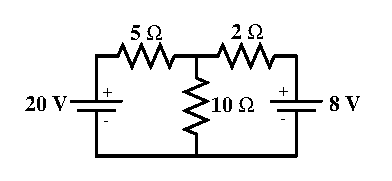
\includegraphics[scale=1]{src/s1s2/en/09_107/fig1}\\
    


  \end{center}





\item Derive EMF equation of d.c. generator.

\item Explain the principle operation of synchronous generator.

\partC

\item \iitem \iitem State and explain Faraday's laws of elecromagnetic induction. \marko{5}

\item Compare electric and magnetic circuits. \marko{5}

\ene

\Or

\newpage

\again

\item \iitem Derive form factor and peak factor of a sine wave.  \marko{5}

\item Three coils, each of resistance of 6 $\Omega$ and inductive reactance 8$\Omega$ are joined in delta across
  400V, 3-phase lines. Calculate the line current and power absorbed. \marko{5}

\ene\ene

\item \iitem Explain the construction and principle of operation  single-phase transformer.

\Or

\item \iitem Explain the construction details of d.c. generator.

\item Explain the principle of operation of induction motor.

\ene\ene\ene



\sectionD

\partA

\iitem What are the advantages and disadvantages of negative feedback? \marko{2}

\item Write RADAR range equation. \marka

\item What is meant by frequency reuse technique? \marko{2}

\partBt

\item Explain briefly about various noises in amplifier.

\item Simplify the following Boolean expression using only NAND gates:

\[ \text{Y} = \bar{\text{A}}\bar{\text{B}}\bar{\text{C}} + \bar{\text{A}}\text{B} \bar{\text{C}} + \text{AB}\bar{\text{C}} + \text{ABC}.\]


\item Explain the principle of GSM. 

\markany{2}{5}{10}

\partCo


\item \iitem \iitem Explain the concept of differential amplifier.  \marko{5}

\item Compare TTL and CMOS logic. \marko{3}

\item List the characteristics of Op-Amp. \marko{2}

\ene

\Or

\item Explain the working of CRO with neat block diagram. \marko{10}

\ene

\newpage

\item \iitem Draw the block diagram of superheterodyne receiver and explain. \marko{10}

\Or

\item \iitem Explain the basic principle of cellular communications. \marko{5}

\item Write short note on GPRS technology. \marko{5}

\ene
\ene
\ene
